\section{Training a neural network}

\mode<presentation>{
\begin{frame}{Where are we?}
    \tableofcontents[currentsection]
\end{frame}
}

\subsection{Recap of gradient-based learning}

\begin{frame}\frametitle{Minimizing the training error}
	Training error $E^T$ for the training set $\left\{(\vec x^{(\alpha)}, y^{(\alpha)}_{T})\right\}$: 
    \begin{equation}
        \ETw = \frac{1}{p} \sum\limits_{\alpha = 1}^p 
					e\tyxwalpha
    \end{equation}
    
    \mode<article>{
    The objective is to minimize the training error w.r.t. the model parameters $\vec w$. That is
    }
    
    \begin{equation}
        \ETw \eqexcl \min_{\vec w} \quad \Rightarrow \quad \vec w^{*} = \argmin_{\vec w} \ETw
    \end{equation}
    
\end{frame}

\begin{frame}\frametitle{Finding the minumum of $\ETw$ iteratively for an \underline{MLP}}

\mode<article>{

Learning from gradient descent is an alternate approach for finding the minimum of a function when the closed-form solution is not available.

}
    \begin{figure}[h]
        \centering
        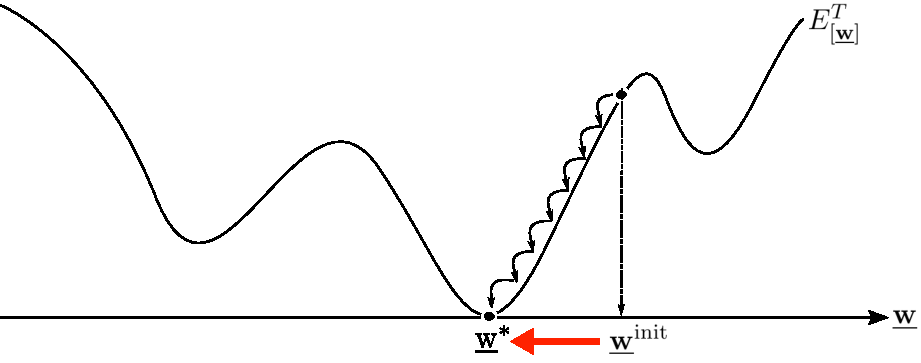
\includegraphics[height=3.cm]{img/section1_fig19}
        \caption{Minimizing the training error iteratively via gradient descent}
        \label{fig:minimize_via_gradient_descent} 
    \end{figure}
    
	\only<1,2>{
    For an MLP:
    \begin{equation}
		w_{ij}^{v'v}(t+1) \quad=\quad w_{ij}^{v'v}(t) 
				\;\;{\color{red}-}\;\;
				\underbrace{\eta}_{ 
						\substack{\text{learning} \\ \text{step} } }
                        \cdot
				\underbrace{\frac{\partial \ETw}{
					\partial {w}_{ij}^{v'v}}}_{
						\substack{
							\text{component of}\\
							\text{\textcolor{red}{gradient vector}} 
			} }
            \label{eq:gradient_descent_mlp}
    \end{equation}
    }
    
    \mode<article>{
    
    The learning step (learning rate) $\eta$ modulates the magnitude of our update. $\eta$ can be treated as a constant but we will also see how the value of $\eta$ can change over time, i.e. $\eta(t)$.
    }
    \only<2>{
    \svspace{-4mm}
    \question{Do you remember why we \underline{subtract} the gradient from $w_{ij}^{v'v}(t)$?}
    }
    
    \mode<article>{
    
    - The gradient describes the slope. Subtracting the gradient aligns with minimizing the function, while adding the gradient would be suitable for maximizing it.
    }
\end{frame}

\subsection{Gradient calculation}

\begin{frame}\frametitle{Recap: connectionist neuron for minimizing quadratic error}
    
    \notesonly{
    Recall from our previous discussion on calculating gradients for a simple connectionist neuron.
    }
    Setting
    \begin{itemize}
       \item \notesonly{minimize quadratic error }$e\tyxw := \frac{1}{2} \left( y_T - y(\vec{x}; \vec w) \right)^2$
       \item \notesonly{use connecitonist neuron as }model class:
            \notesonly{\begin{equation}}
            \slidesonly{$}
                y(\vec x; \vec w) := 
                f \Big(\; \sum_{j=0}^{N} {w}_{j} {x}_j
                \; \Big){}
                = f \left( h (\vec x; \vec w)\right)
            \slidesonly{$}
            \notesonly{\end{equation}}
    \end{itemize}
    
    \only<1>{
    \begin{equation}
    		w_{j}(t+1) \quad=\quad w_{j}(t) 
				\;\;{\color{red}-}\;\;
				\underbrace{{\eta}}_{ 
						\substack{\text{learning} \\ \text{step} } }
                        \cdot
				\underbrace{\frac{\partial \ETw}{
					\partial {w}_{j}}}_{
						\substack{
							\text{component of}\\
							\text{\textcolor{red}{the gradient}} 
			} }
    \end{equation}
    }
    \only<2>{
	\begin{align}
		\frac{\partial \ETw}
			{\partial {w}_{j}}
		\;=\;& \frac{1}{p} \sum_{\alpha=1}^p	\underbrace{
			\textcolor{blue}{
			\frac{\partial e\tyxwalpha}{\partial 
					y(\vec{x}^{(\alpha)}, \vec{w})} }}_{
						\substack{\text{factor depending} \\
							\text{on cost function}}}
				  \;\cdot \underbrace{
			\textcolor{orange}{
			\frac{\partial y(\vec{x}^{(\alpha)}; \vec{w})}{
					\partial {w}_{j}}} }_{
						\substack{\text{factor depending on} \\
							\text{model class}\\
                            \text{(e.g. perceptron, MLP)}}}\\
            \intertext{then specifically for \textcolor{blue}{quadratic error} and the \textcolor{orange}{connectionist neuron}:}
            \;=\;& \frac{1}{p} \sum_{\alpha=1}^p
            \textcolor{blue}{(y{(\vec{x}^{(\alpha)}; \vec{w}) - y_T^{(\alpha)})}}
            \cdot
            \textcolor{orange}{
            f'(h(\vec x^{(\alpha)}; \vec w))
            \cdot
            x_{j}
            }
	\end{align}
    }

\end{frame}

\begin{frame}\frametitle{Computing gradients for an MLP}

    \mode<presentation>{
    \begin{equation*}
        w_{ij}^{v'v}(t+1) \quad=\quad w_{ij}^{v'v}(t) 
            \;\;{\only<1>{\color{red}}-}\;\;
            \underbrace{\eta}_{ 
                    \substack{\text{learning} \\ \text{step} } }
                    \cdot
            \underbrace{\frac{\partial \ETw}{
                \partial {w}_{ij}^{v'v}}}_{
                    \substack{
							\text{component of the }\\
                        \text{\only<1>{\textcolor{red}}{gradient vector}} 
        } }
    \end{equation*}
    
    \only<1>{
    
    \begin{figure}[ht]
     \centering
     \savebox{\imagebox}{
	 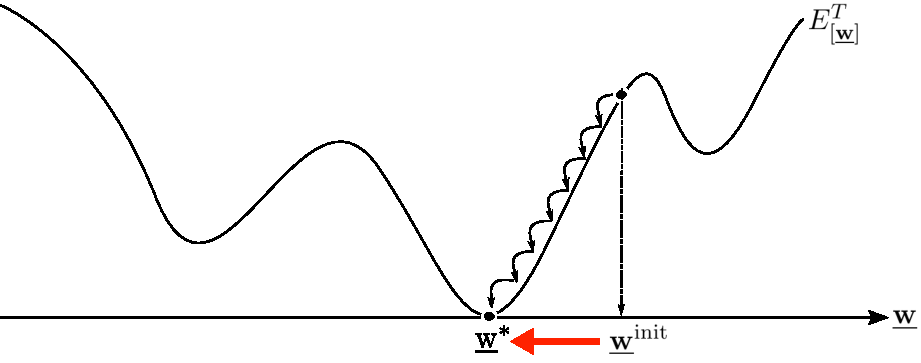
\includegraphics[trim=150 0 0 0,clip,height=2.5cm]{img/section1_fig19}}%
     \begin{subfigure}[t]{0.35\textwidth}
         \centering
         \usebox{\imagebox}% Place largest image
     \end{subfigure}
     \hspace{7mm}
     \begin{subfigure}[t]{0.49\textwidth}
         \centering
         \raisebox{\dimexpr.5\ht\imagebox-.5\height}{% Raise smaller image into place
         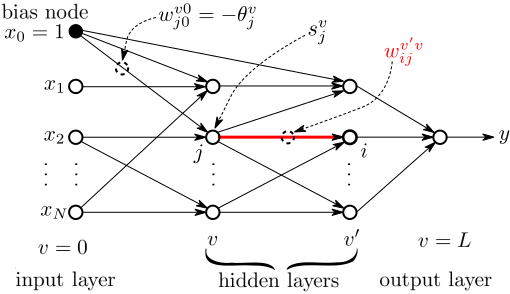
\includegraphics[width=0.99\textwidth]{img/section1_fig14_ij}
         }
     \end{subfigure}
    \end{figure}
    }
    \only<2>{
	\begin{align}
		\frac{\partial \ETw}
			{\partial {w}_{ij}^{v'v}}
		\;=\;& \frac{1}{p} \sum_{\alpha=1}^p	\underbrace{
			\textcolor{blue}{
			\frac{\partial e\tyxwalpha}{\partial 
					y(\vec{x}^{(\alpha)}, \vec{w})} }}_{
						\substack{\text{factor depending} \\
							\text{on cost function}}}
				  \;\cdot \underbrace{
			\textcolor{orange}{
			\frac{\partial y(\vec{x}^{(\alpha)}; \vec{w})}{
					\partial {w}_{ij}^{v'v}}} }_{
						\substack{\text{factor depending on} \\
							\text{model class}\\
                            \text{(e.g. perceptron, MLP)}}}
	\end{align}
    }
    }
\end{frame}

    
    \mode<article>{
    \begin{figure}[h]
        \centering
        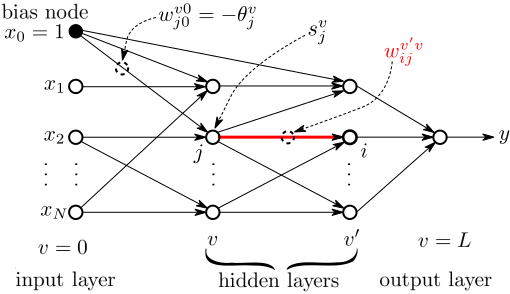
\includegraphics[height=3cm]{img/section1_fig14_ij}
        \caption{Example MLP architecture}
        \label{fig:example_mlp}
    \end{figure}
    
    \eqref{eq:gradient_descent_mlp} shows us how gradients are used for iteratively finding the minimum of the training error.
    The layered structure of an MLP implies that computing the gradient requires a more involved application of the chain rule. The backpropagation algorithm exploits the chain rule to efficiently compute the gradients for an MLP.
    }
    
